\documentclass[10pt,a4paper]{report}
\usepackage[latin1]{inputenc}
\usepackage{amsmath}
\usepackage{amsfonts}
\usepackage{amssymb}
\usepackage{graphicx}
\graphicspath{{./Figures/}}
\usepackage{hyperref}
\usepackage{multicol}
\usepackage[margin=0.5in]{geometry}
\usepackage{tikz}
\usepackage{romannum}
\usetikzlibrary{arrows,shapes.gates.logic.US,shapes.gates.logic.IEC,calc}


\begin{document}

\centering {
\includegraphics[scale=0.07]{IITH.png}} \vspace{3mm}\\ \raggedleft Name: Bole Manideep\vspace{2mm}\\ \raggedleft Roll No.: FWC22026\vspace{2mm}\\ \raggedright Sep 2022 \hspace{12cm} \raggedleft manideepbole312@gmail.com \vspace{10mm}
\\ \centering \Large \textbf{MATRIX ASSIGNMENT} \normalsize \vspace{15mm}

\begin{multicols}{2}

\raggedright \large \underline{Problem Statement:} \normalsize \vspace{5mm}
\\ \hspace{2cm} For a given parallelogram ABCD, show that for any point 'P' inside the parallelogram,\\ \vspace{5mm}\raggedright \romannum{1}. $Ar(\Delta APB)+Ar(\Delta PCD) = \frac{1}{2}Ar(ABCD)$ \vspace{5mm} \\ 
\raggedright \romannum{2}. $Ar(\Delta APB)+Ar(\Delta PCD)=Ar(\Delta APD)+Ar(\Delta PCB)$ \vspace{2mm} \\ \centering 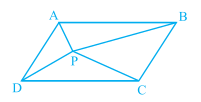
\includegraphics[scale=1.1]{Question.png} \vspace{2mm} \\ \raggedright \large \underline{Solution:} \normalsize \\ \vspace{1mm} \raggedright Given a Parallelogram 'ABCD' with a interior point 'P'\\ We Know That,\\ \raggedright \hspace{2cm} Ar(\Delta le) = \frac{1}{2}*Base*Height \hspace{1.3cm} (eq 1) \\ \hspace{2cm} \raggedright Ar($||$gm) = Base*Height \hspace{2cm} (eq 2) \vspace{3mm}
\\ \raggedright \underline{(\romannum{1}) $Ar(\Delta APB)+Ar(\Delta PCD) = \frac{1}{2}Ar(ABCD):$} \\ \vspace{1mm} \raggedright \hspace{1cm} Let us consider a line 'EF' drawn parallel to 'AB' and 'CD' that is passing through the point 'P' as shown in the Fig.1.\\
\vspace{2mm} \centering 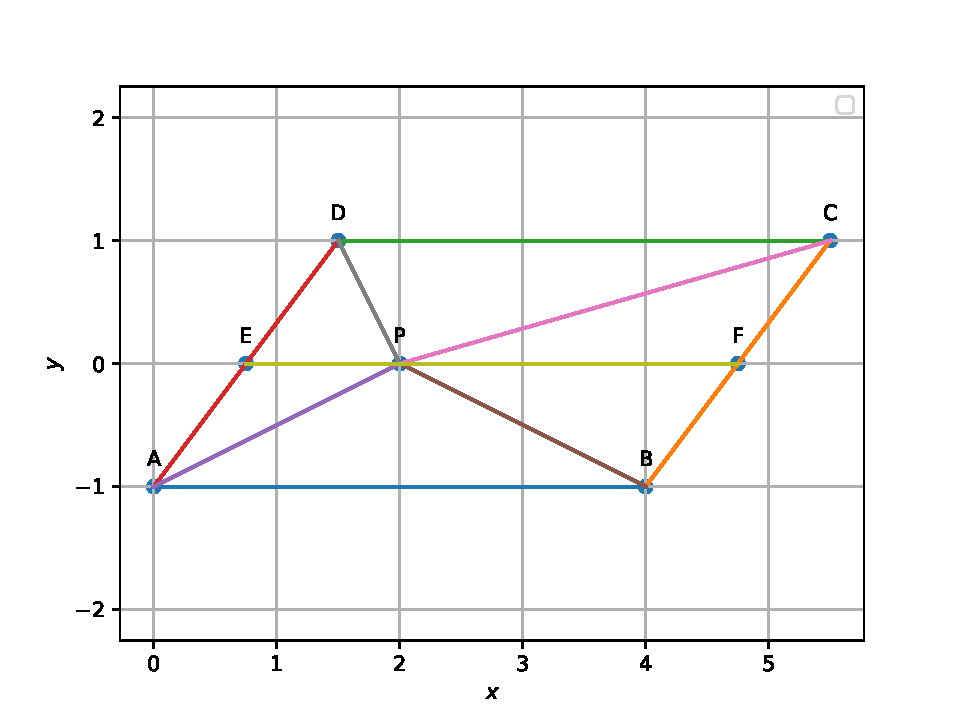
\includegraphics[scale=0.4]{fig1.pdf} \\ \underline{Fig.1} \\
\raggedright Now 'EFCD' becomes a parallelogram with Triangle PCD inside it. 
\\ Parallelogram EFCD and Triangle PCD have the same base 'CD'.
\\If we consider a perpendicular from point 'P' to line 'CD', it becomes the height h for both $||$gm EFCD and \Delta le PCD. \\ From "eq 1" and "eq 2",\\
\raggedright \hspace{2cm} Ar(\Delta PCD) = \frac{1}{2}*CD*h \\ \raggedright \hspace{2cm} Ar($||$gm EFCD) = CD*h \\ \raggedright \vspace{1mm} \hspace{1cm} \Rightarrow Ar(\Delta PCD) = \frac{1}{2}*Ar(||gm EFCD) \hspace{1cm} (eq 3) \\ \raggedright Similarly, \\ \raggedright \vspace{1mm} \hspace{1cm} \Rightarrow Ar(\Delta APB) = \frac{1}{2}*Ar(||gm ABFE) \hspace{1cm} (eq 4) \\ \raggedright On adding RHS of "eq3" and "eq4" we get total area of Paralleogram ABCD, \\ \vspace{3mm} \raggedright  \therefore Ar(\Delta APB)+Ar(\Delta PCD) = \frac{1}{2}Ar(||gm ABCD) \hspace{5mm} (eq 5) \vspace{4mm}
\\ \raggedright \underline{(\romannum{2}) $Ar(\Delta APB)+Ar(\Delta PCD)=Ar(\Delta APD)+Ar(\Delta PCB):$} \\
\vspace{2mm} \hspace{1cm} Now let's consider a line 'GH' drawn parallel to 'AD' and 'BC' that is passing through the point 'P' as shown in the Fig.2.\\ \centering
\vspace{2mm} 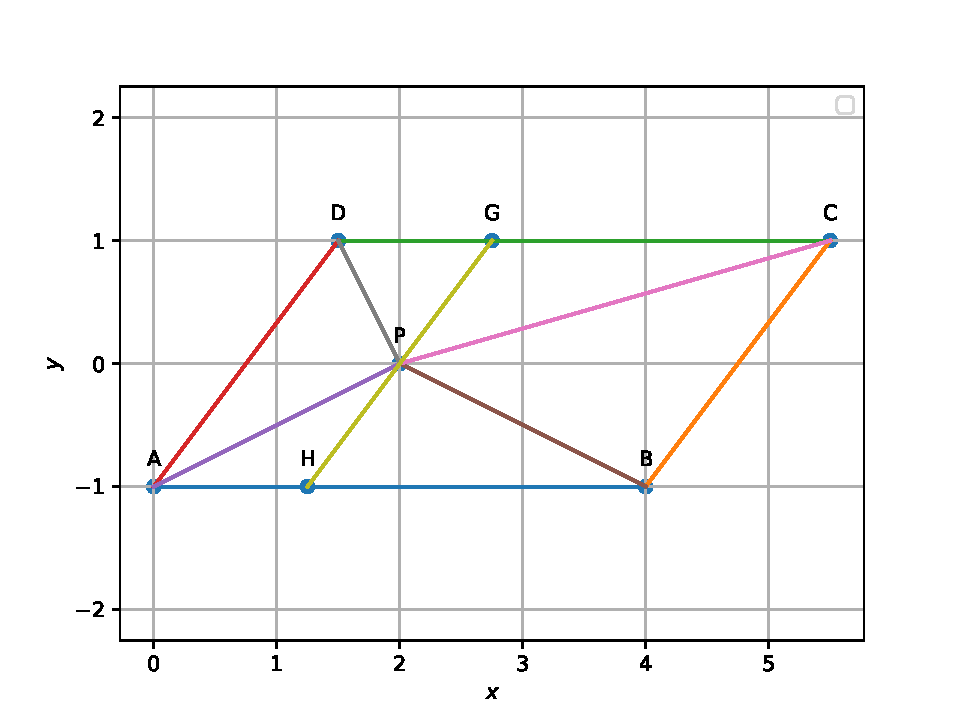
\includegraphics[scale=0.4]{fig2.pdf} \\ \underline{Fig.2} \vspace{3mm} \\ \raggedright Similarly, from the above proof we can state that, \\ \raggedright \Rightarrow Ar(\Delta APD)+Ar(\Delta PCB) = \frac{1}{2}Ar(||gm ABCD) \hspace{5mm} (eq 6) \vspace{4mm} \\ \raggedright On comparing "eq 5" and "eq 6", \vspace{2mm}\\ \therefore Ar(\Delta APB)+Ar(\Delta PCD)=Ar(\Delta APD)+Ar(\Delta PCB) \\ \vspace{2mm} \centering "Hence Proved"
\vspace{3cm}


\end{multicols}

\end{document}
